\chapter{Planificación}

Como ya se ha mencionado, el proyecto seguirá las prácticas y principios del enfoque ágil, que se fundamenta en los 17 principios delineados en \href{https://agilemanifesto.org/iso/es/manifesto.html}{el manifiesto ágil}. Ágil no es una metodología ni un marco de trabajo, sino una mentalidad que permite a las organizaciones ser más receptivas al cambio. Estos principios están diseñados para asegurar la satisfacción del cliente a través de la entrega temprana y continua de valor, con un fuerte enfoque en la excelencia técnica, el buen diseño, la planificación y la simplicidad.

Estos principios no son solo una referencia teórica, sino que se han aplicado con éxito en proyectos reales y actuales, de acuerdo con~\cite{berlas2024software}. Este informe presenta una revisión completa de la investigación publicada sobre las métricas de software en el desarrollo ágil y resalta su efectividad en diversos contextos, incluyendo pequeñas y medianas empresas.

\begin{itemize}
    \item \textbf{¿Se está usando enfoques ágiles?} El informe indica que los enfoques ágiles son ampliamente utilizados en la industria del software, permitiendo a los equipos de desarrollo trabajar iterativamente y responder rápidamente a las necesidades del cliente.
    \item \textbf{¿Esto verdaderamente funciona?} Según el informe, los enfoques ágiles han demostrado ser eficaces en diversos tipos de proyectos a cualquier escala proporcionando beneficios como la reducción del tiempo de comercialización, mayor satisfacción del cliente y disminución de los costos de desarrollo.
\end{itemize}    

Para garantizar la aplicación coherente de estos principios, la memoria debe desarrollarse de forma iterativa e incremental, con actualizaciones a medida que avanza el proyecto y se toman decisiones. Esto nos permite evaluar continuamente cómo estamos añadiendo valor al proyecto.

En este punto, es dónde las historias de usuario y los objetivos iniciales se convierten en la guía para el desarrollo del proyecto. Las mismas también forman parte de la planificación, pues, son las que garantizan la entrega y calidad continua de un producto.

\section{Entrega y calidad continua}

Para asegurar la calidad del proyecto y la entrega continua, se han empleado una serie de herramientas y enfoques que se han integrado en el flujo de trabajo tanto local como remoto.

La documentación del proyecto es una de las partes más importantes (junto con el código) del trabajo de fin de grado si no la que más por lo que se ha de poner especial atención en que esta sea de calidad y cumpla con los requisitos establecidos por tutor y tribunal. Para dar cuenta de esto, la memoria se ha elaborado en \href{https://www.latex-project.org/}{\LaTeX{}} que es un sistema de composición tipográfica de alta calidad; incluye funciones diseñadas para la producción de documentación técnica y científica además de estar disponible como software libre.

Para complementar, comprobar y mejorar la calidad de la documentación se han usado una serie de herramientas que se han integrado en el flujo de trabajo local tanto con extensiones de (\href{https://code.visualstudio.com/}{\textit{Visual Studio Code}}) como con herramientas ejecutadas en la línea de comandos.

En cuanto a flujos de trabajo remotos en \textit{GitHub} se han implementado uno específico para la memoria. Este flujo de trabajo se activa en cada push y se encarga de realizar verificaciones gramaticales y ortográficas con \href{https://github.com/sylvainhalle/textidote}{\textit{TeXtidote}} de la cual se sube un informe y si pasa estas verificaciones de forma satisfactoria se sube la memoria compilada en formato PDF a modo de artefacto. Este flujo de trabajo remoto junto con el local garantizan la calidad de la documentación.

Ese artefacto generado tras acabar cada \textit{milestone} o hito podría ser perfectamente entregable a un cliente final a modo de entrega continua para que vea el progreso del proyecto. A mayores, hacemos referencia al tercer principio del \href{https://agilemanifesto.org/iso/es/principles.html}{manifiesto ágil} que dice: \textit{``Entregar software funcional frecuentemente, entre dos semanas y dos meses, con preferencia al periodo de tiempo más corto''}. Además, los flujos de trabajo remotos (en \textit{GitHub}) y locales promueven el noveno principio que hace referencia a la atención continua a la excelencia técnica y el buen diseño.

\section{Metodologías para el seguimiento del desarrollo}

En esta sección se documentarán las metodologías empleadas para el seguimiento del desarrollo del proyecto. Al aplicar estas metodologías se ha conseguido una mayor eficiencia en la gestión del tiempo y de los recursos, así como una mayor calidad en la documentación y en el código fuente. Además, se explicarán las herramientas utilizadas para el control de versiones y el alojamiento del repositorio remoto del proyecto.

\subsection{\textit{Git y GitHub}: control de versiones y colaboración}

Para el control de versiones se ha empleado \textit{git} que es un sistema de control de versiones que permite llevar un control de los cambios en el código fuente.

Para la colaboración y hospedaje del código fuente se ha hecho en \textit{GitHub}, una plataforma que permite alojar proyectos de \textit{software} y colaborar en ellos. En \textit{GitHub} tenemos diferentes funcionalidades que han sido de ayuda para el desarrollo del proyecto.

\textbf{El repositorio del proyecto se puede encontrar en la siguiente dirección: \url{https://github.com/danigonzser/proyecto-tfg}.}

La transparencia y accesibilidad de GitHub facilitan la comunicación constante y la colaboración del equipo, apoyando los principios ágiles de la colaboración diaria entre desarrolladores y clientes, y de la construcción de proyectos en torno a individuos motivados.

En GitHub se integran diferentes herramientas que permiten llevar un control del desarrollo del proyecto. A continuación, se describen algunas de las funcionalidades más importantes.

\subsubsection{\textit{Issues}}

A lo largo del proyecto se van a ir encontrando diferentes problemas que se han de resolver. Para llevar un control de los mismos se han ido creando \textit{issues}. Estos no solo son descripciones de los problemas que se quieren resolver, sino que pueden ser una buena medida para saber si se progresa hacia el \textit{milestone} o no.

\begin{figure}[H]
    \caption{Captura de pantalla del listado de \textit{issues} del repositorio del proyecto de \textit{GitHub}.}
    \centering
    \vspace*{0.5cm}
    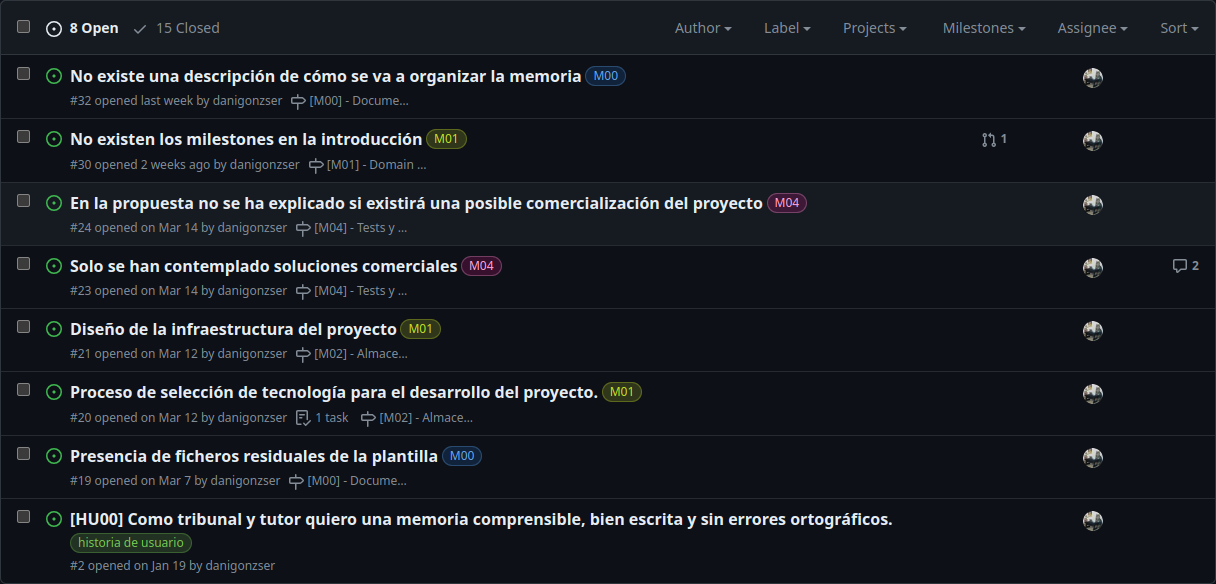
\includegraphics[scale=0.2]{figuras/github_issues.png}
\end{figure}

Existe un acceso a la documentación de la metodología seguida que se puede consultar en el siguiente \href{https://github.com/danigonzser/proyecto-tfg/issues?q=is%3Aissue+is%3Aclosed}{enlace}, aquí se encuentra el registro completo de los \textit{issues} cerrados, que ilustran el proceso de resolución de problemas y la evolución del proyecto. A continuación, se muestra un pantallazo de los \textit{issues} cerrados:

\begin{figure}[H]
    \caption{Pantallazo del listado de issues cerradas.}
    \centering
    \vspace*{0.5cm}
    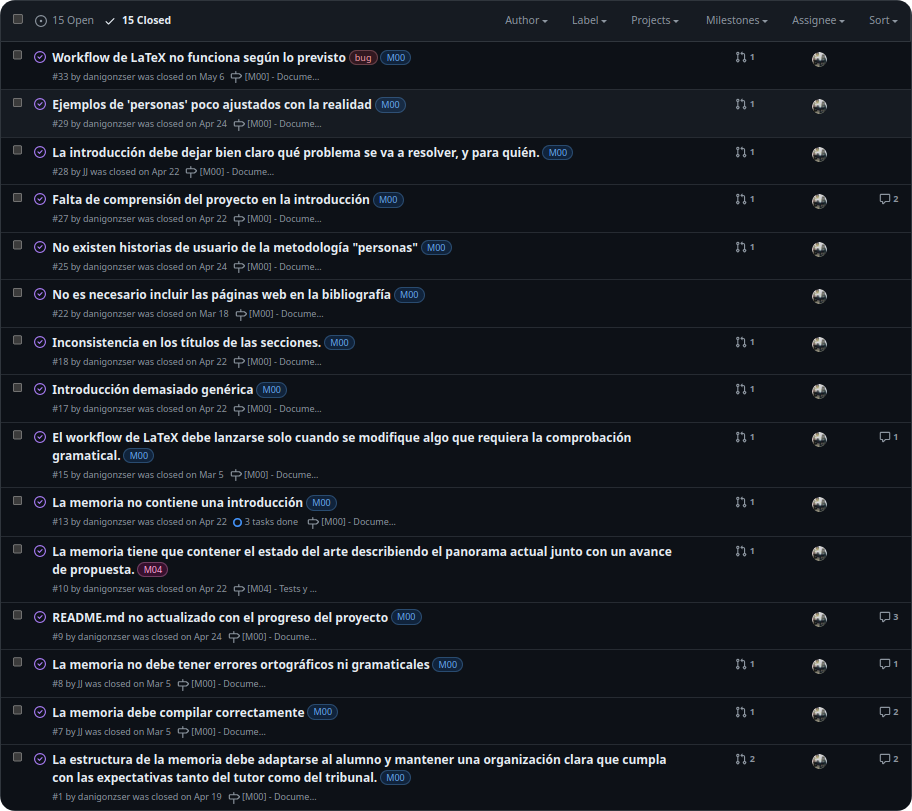
\includegraphics[scale=0.2]{figuras/listado_issues_cerradas.png}\label{fig:figuras/listado_issues_cerradas.png}
\end{figure}

\subsubsection{Pull requests}

Los pull requests son una forma de proponer cambios en el código fuente sin que estos se apliquen directamente al código fuente o rama principal sin una aprobación previa. Estos son una manera de revisar que los cambios mantengan la excelencia técnica y calidad del proyecto apoyando al noveno principio del manifiesto ágil.

Para proteger la rama principal o \textit{master} de cambios no deseados se han configurado una serie de reglas que impiden la integración de cambios a menos que:

\begin{itemize}
    \item Los tests deben de haberse realizado de manera exitosa.
    \item Que la rama esté actualizada.
    \item Que las conversaciones hayan sido resueltas.
\end{itemize}

A continuación se muestra una captura de pantalla de la lista de \textit{pull requests} del proyecto hasta el momento.

\begin{figure}[H]
    \caption{Captura de pantalla del listado de \textit{pull requests} del repositorio del proyecto de \textit{GitHub}.}
    \centering
    \vspace*{0.5cm}
    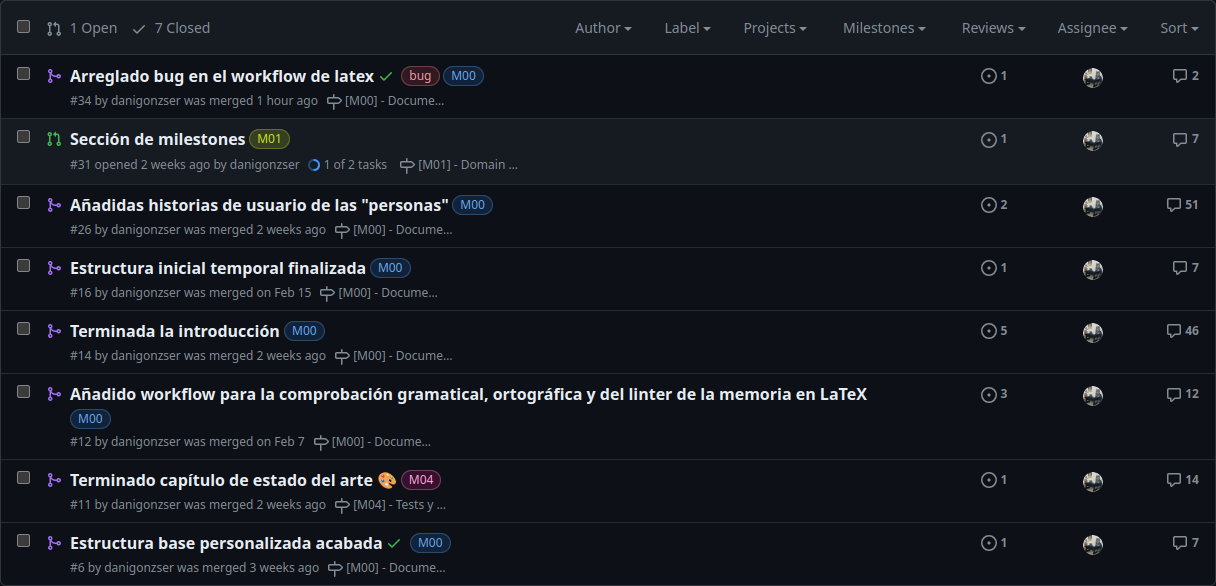
\includegraphics[scale=0.2]{figuras/listado_pull_requests_github.png}
\end{figure}

En la figura se puede apreciar que se han abierto 8 \textit{pull requests} hasta el momento. Los que están en color morado son los \textit{pull requests} que ya han sido integrados en la rama principal y el que está en color verde es el que todavía no está integrado.

\begin{figure}[H]
    \caption{Captura de pantalla del contenido de una \textit{pull request}.}
    \centering
    \vspace*{0.5cm}
    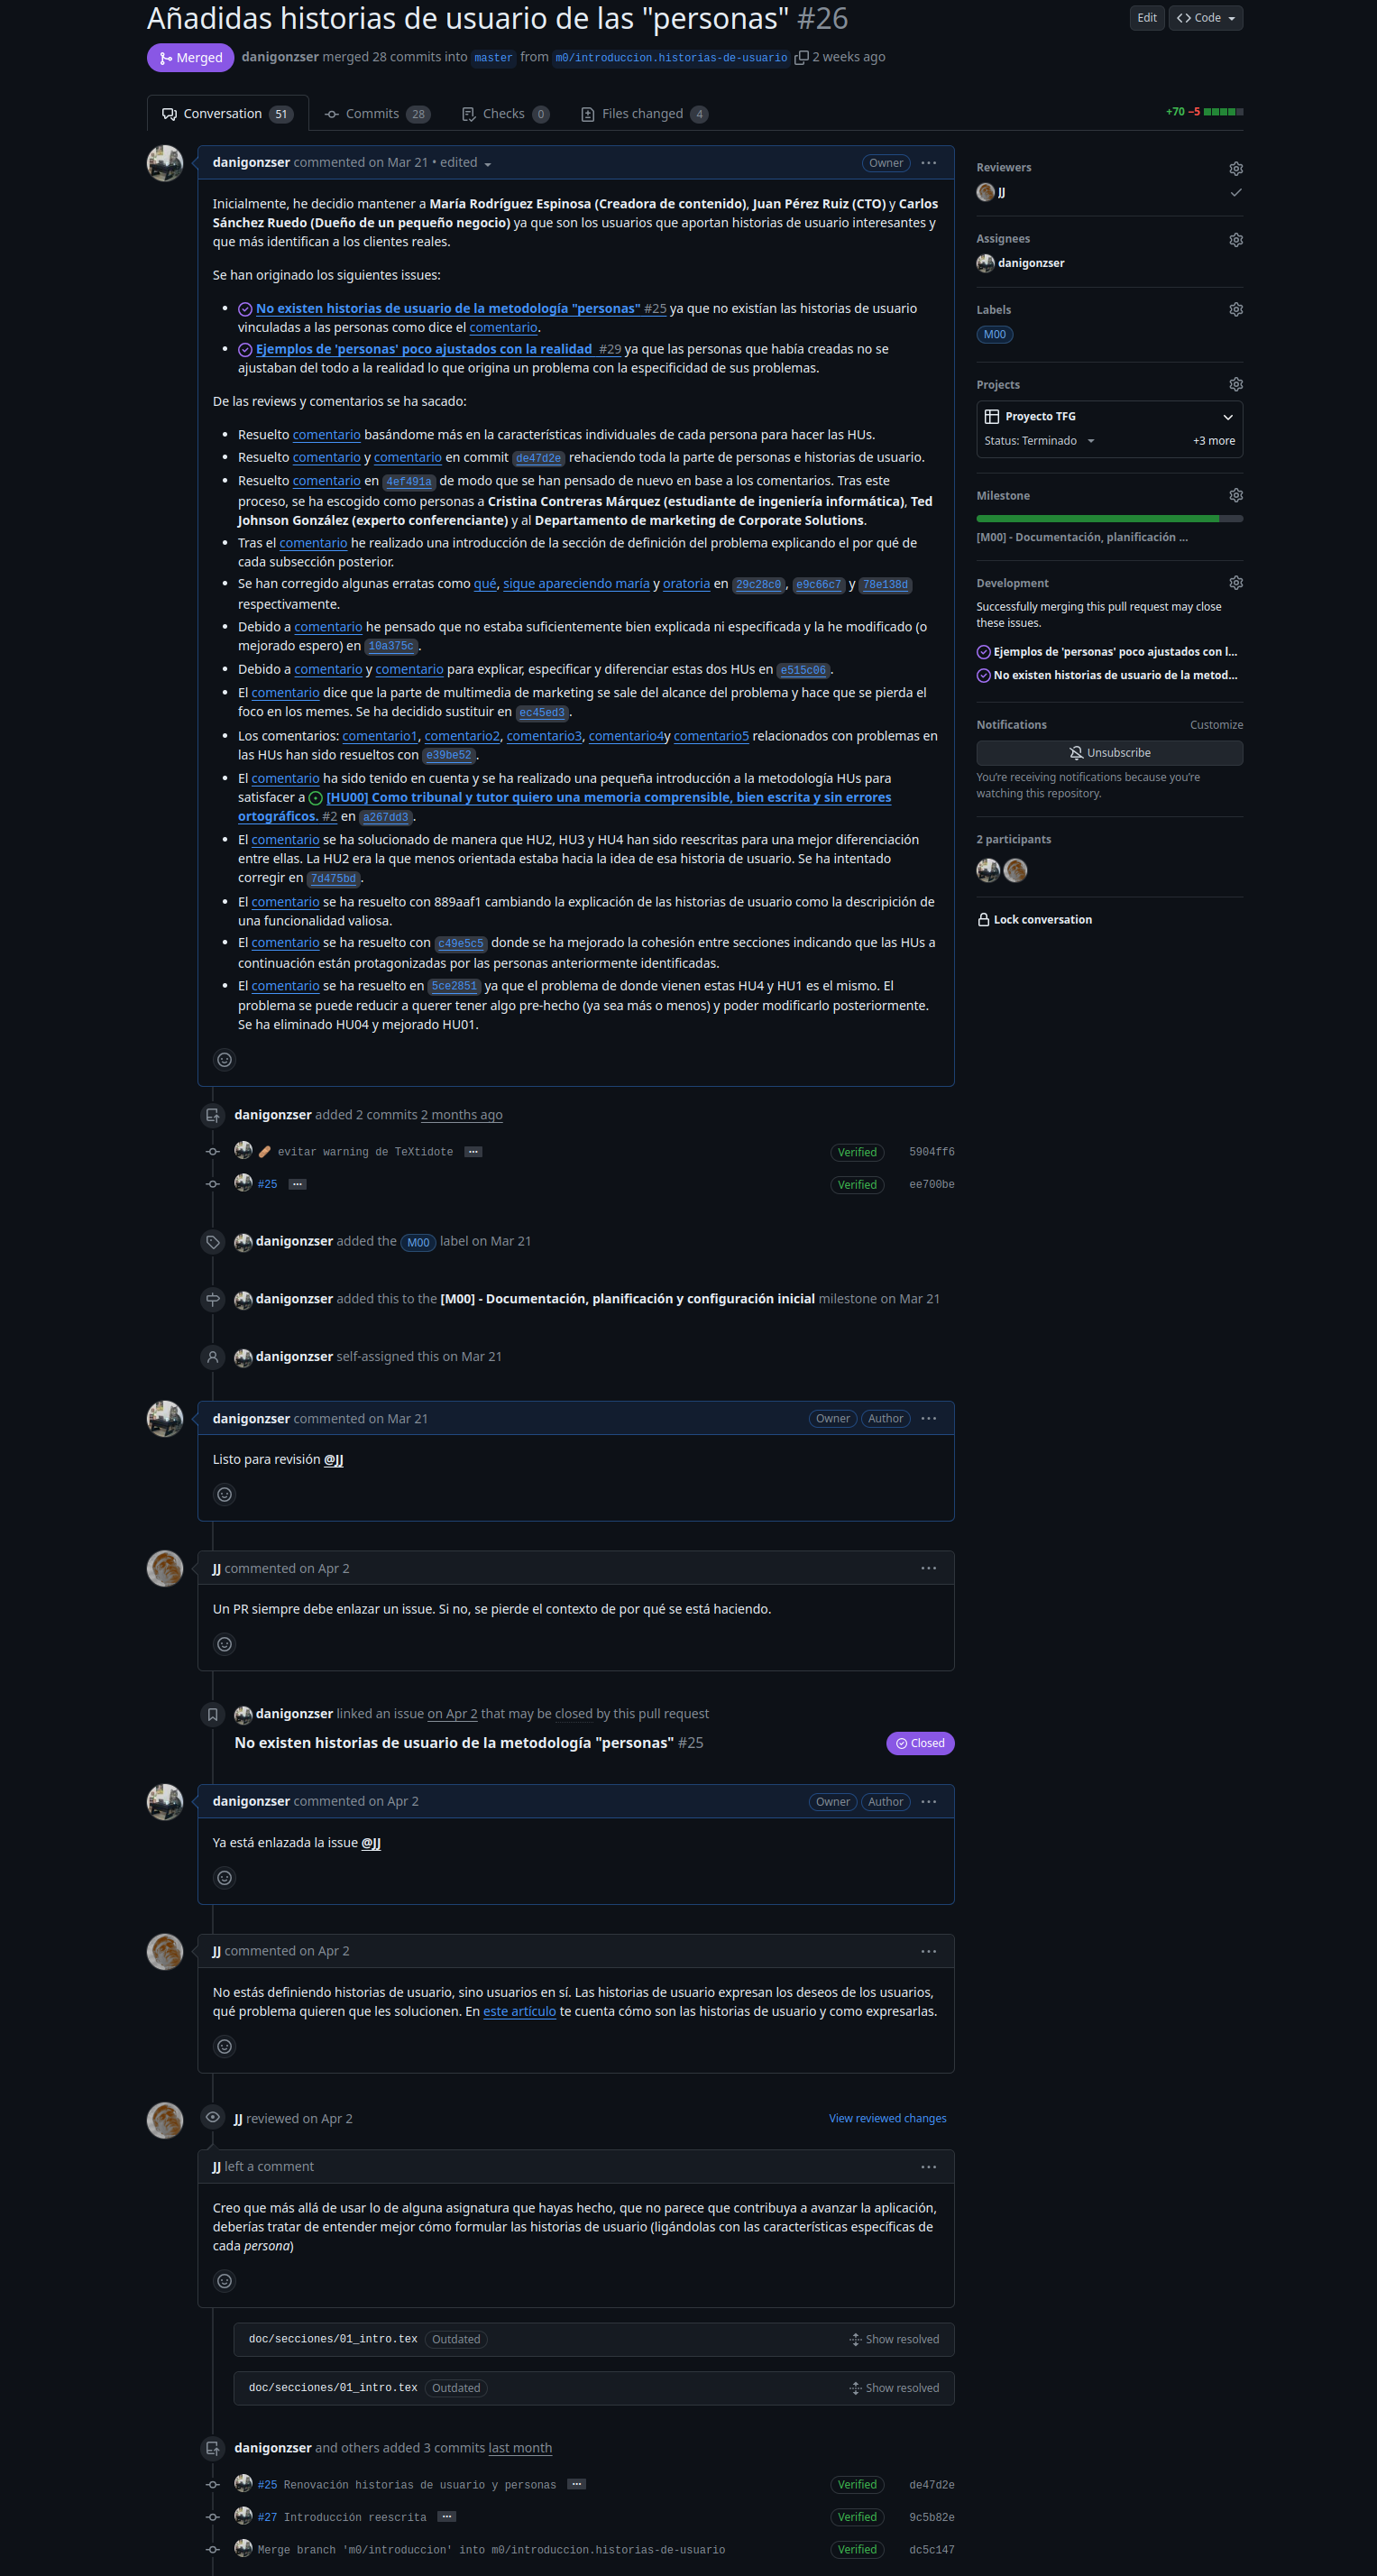
\includegraphics[scale=0.1]{figuras/pull_request_github.png}\label{fig:contenido_pull_request}
\end{figure}

Como se puede ver en la figura~\ref{fig:contenido_pull_request} el estado de la \textit{pull request} es \textit{merged} lo que significa que ya ha sido integrado en la rama principal. Más abajo se puede ver el cuerpo de la misma donde residen todas las \textit{issues} que han sido creadas y consecuentemente resueltas con esta \textit{pull request}. Más abajo se puede ver el historial de commits y de conversaciones que se han ido originando a lo largo de la resolución. Al final de la imagen es donde podemos ver esas conversaciones que deben ser resueltas antes de integrar los cambios en la rama principal. Finalmente, a la derecha se muestran detalles como el revisor, el asignado, las etiquetas, el proyecto al que pertenece, el \textit{milestone} y las \textit{issues} relacionadas.

\subsubsection{\textit{Projects}: tablero kanban}

La funcionalidad de projects de \textit{GitHub} se ha utilizado para llevar un control de la evolución y progreso de los \textit{issues} y \textit{pull requests}. Se ha implementado un tablero \textit{kanban} como se puede ver en la imagen~\ref{fig:tablero_kanban} que permite ver de un vistazo el estado de los \textit{issues} y \textit{pull requests}. Esto es muy útil para saber si se progresa, cómo se están resolviendo los problemas y si se está cumpliendo con los objetivos marcados. Además, está relacionado con los principios ágiles al promover la auto-organización, entrega frecuente y temprana y atención continua.

\begin{figure}[H]
    \caption{Captura de pantalla del tablero \textit{kanban} en la sección de \textit{projects} de \textit{GitHub}.}
    \centering
    \vspace*{0.5cm}
    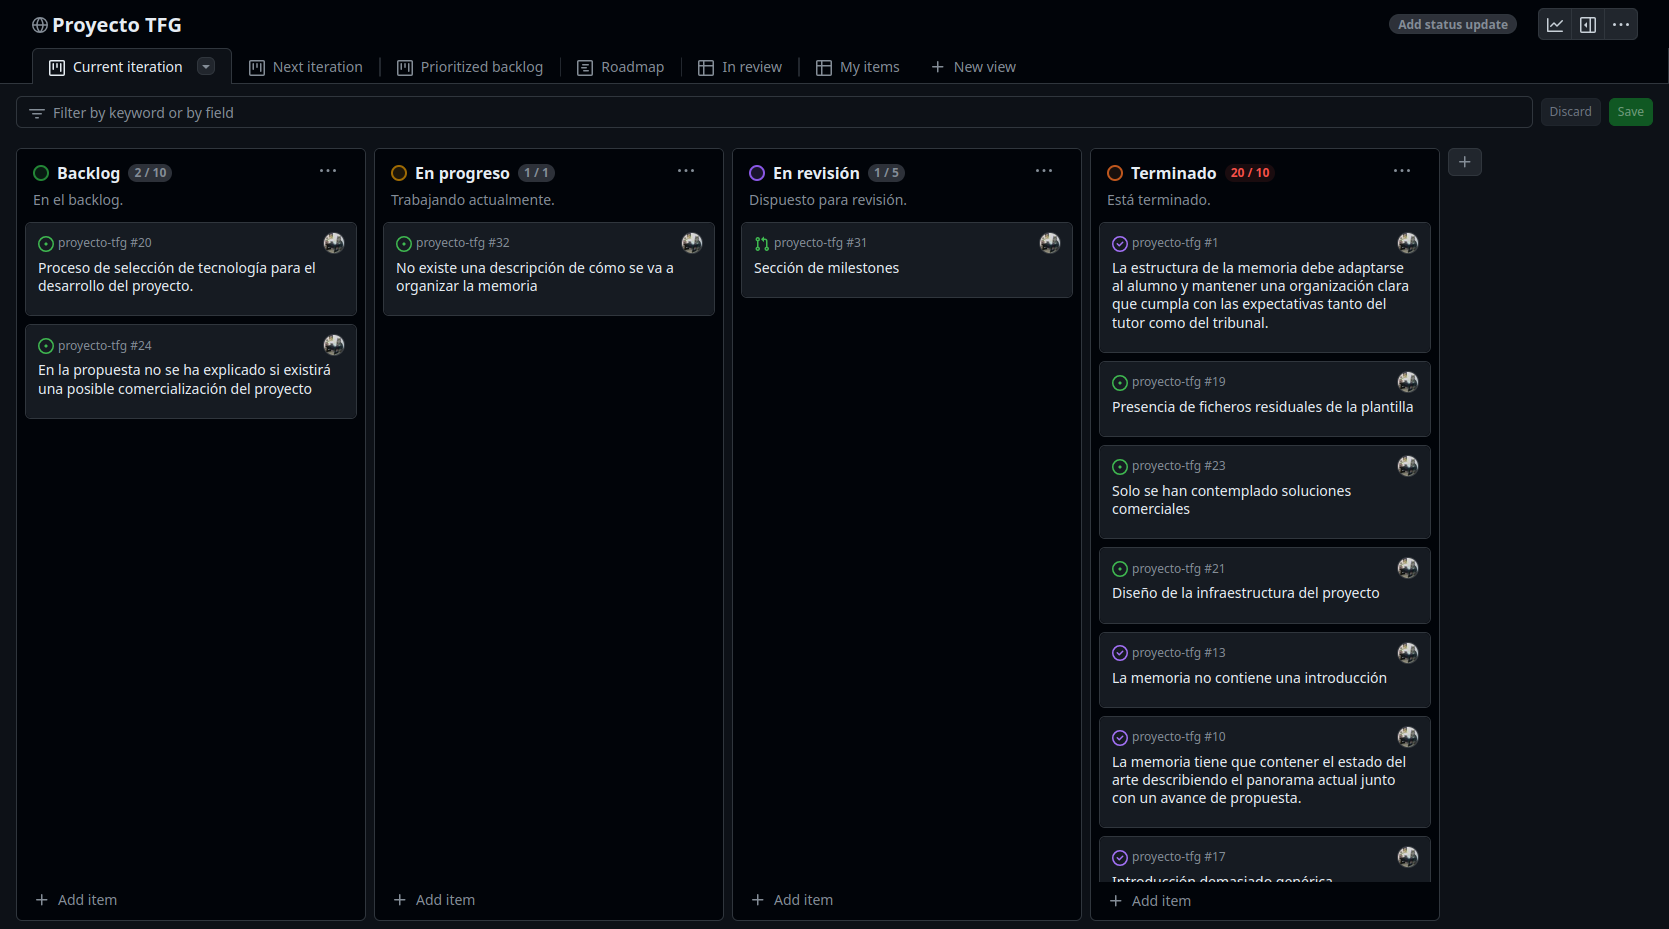
\includegraphics[scale=0.2]{figuras/projects_github.png}\label{fig:tablero_kanban}
\end{figure}

\section{Temporización}

La gestión de tiempo y recursos en nuestro proyecto se realiza mediante el uso de \textit{milestones} en GitHub, que son el equivalente a los \textit{sprints} en el enfoque ágil. Los \textit{milestones} se han creado a partir de las historias de usuario, asegurando que cada fase del proyecto esté orientada a cumplir con las necesidades y expectativas del usuario final. Un conjunto específico de \textit{issues} puede ser incluido en un \textit{milestone} y, al finalizar el \textit{sprint}, estos \textit{issues} deben estar resueltos. Al concluir el \textit{milestone}, debe resultar en un producto mínimamente viable y en nuestro repositorio vamos a etiquetarlos como nueva versión del proyecto.

\subsection{Milestones}

\begin{itemize}
    \item \textbf{[M00] \- Documentación, planificación y configuración inicial}
    \begin{itemize}
        \item \textit{Descripción}: Este \textit{milestone} abarca la creación de la documentación inicial, la planificación del proyecto y la configuración de las herramientas necesarias.
    \end{itemize}

    \item \textbf{[M01] \- Domain Driven Design}
    \begin{itemize}
        \item \textit{Descripción}: Enfocado en la implementación del diseño dirigido por el dominio (DDD).
    \end{itemize}
\end{itemize}

A partir de aquí, los \textit{milestones} se irán definiendo y ajustando conforme avance el proyecto, siguiendo los principios del desarrollo ágil que promueven la adaptación continua y la respuesta al cambio. Los \textit{milestones} sucesivos se centrarán en la implementación.